\documentclass[a4paper, 12pt]{article}
\usepackage[a4paper,top=1.5cm, bottom=1.5cm, left=1cm, right=1cm]{geometry}

% Работа с русским языком
\usepackage[utf8]{inputenc}
\usepackage{mathtext}                % русские буквы в формулах
\usepackage[english, russian]{babel} % локализация и переносы

\usepackage{graphicx}   % Вставка изображений
\usepackage{float}      % "Плавающие" изображения3
\usepackage{wrapfig}    % Обтекание фигур (таблиц, картинок и прочего)
\usepackage{subfig}
\graphicspath{ {./images/} }

\usepackage{tabularx}
\usepackage{multirow}
\usepackage{booktabs}
\usepackage{amsmath}
\usepackage{amsfonts}
\usepackage{indentfirst}
\usepackage{longtable}
\graphicspath{{pictures/}}
\usepackage{natbib}
\usepackage{bm}

\newcommand{\figref}[1]{(См. рис. \ref{#1})}
\newcommand{\secref}[1]{(См. раздел. \ref{#1})}

\newcommand{\angstrom}{\text{\normalfont\AA}}
\newcommand{\e}[1]{\text{$\cdot10^{#1}$}}
\newcommand{\m}{\; м}
\newcommand{\mm}{\; мм}
\newcommand{\um}{\; мкм}
\newcommand{\A}{\; А}
\newcommand{\uV}{\; мкВ}
\newcommand{\cels}{\; ^\circ С}

%%% Колонтитулы
\usepackage{titleps}
\newpagestyle{main}{
	\setheadrule{0.4pt}
	\sethead{Отчёт о выполнении лабораторной работы 1.1}{}{}
	\setfootrule{0.4pt}                       
	\setfoot{ФРКТ МФТИ, 2024}{}{\thepage} 
}
\pagestyle{main}  

\begin{document}
    \begin{titlepage}
	\begin{center}
            {\large МОСКОВСКИЙ ФИЗИКО-ТЕХНИЧЕСКИЙ ИНСТИТУТ (НАЦИОНАЛЬНЫЙ ИССЛЕДОВАТЕЛЬСКИЙ УНИВЕРСИТЕТ)}
	\end{center}
 
	\begin{center}
		{\large Физтех-школа радиотехники и компьютерных технологий}
	\end{center}
	
	\vspace{8cm}
	{\LARGE
		\begin{center}
                {\bf Отчёт о выполнении лабораторной работы 1.1}\\
                Экспериментальная проверка уравнения Эйнштейна для фотоэффекта и определение постоянной Планка
		\end{center}
	}
	\vspace{4cm}
	\begin{flushright}
		{\Large Авторы: \\ 
        Тихонов Дмитрий Романович, \\ студент группы Б01-206а \\
        Павловский Кирилл Михайлович, \\ студент группы Б01-206а}
	\end{flushright}
	\vspace{4cm}
	\begin{center}
		\Large Долгопрудный, 2024
	\end{center}
    \end{titlepage}


    \section{Введение}

    \noindent \textbf{Цель работы:} исследовать зависимость величины фототока от задерживающего потенциала и частоты падающего излучения; вычислить величину постоянной Планка. \\
	

    \noindent \textbf{В работе используются:} фотоэлемент Ф-25, призменный монохроматор УМ-2, неоновая лампа, лампа накаливания К-12, вольметры GDM-8145, блок питания.
    
    \section{Теоретические сведения}

    \section{Теоретическое введение}
	
	Фотоэффект -- явление испускания электронов фотокатодом, облучаемым светом,  Это явление хорошо объясняется фотонной теорией света. Взаимодействие монохроматического света с веществом можно описывать как взаимодействие с веществом частиц, называемых фотонами, которые обладают энергией $\hbar \omega$ и импульсом $\hbar\omega/c$. При столкновении фотона с электроном фотокатода энергия фотона полностью передается электрону, и фотон прекращает свое существование. Энергетический баланс этого взаимодействия для вылетающих электронов описывается уравнением
	
	\begin{equation}
        \hbar \omega = E_{max} + W
        \label{eq:energy}
	\end{equation}
	
	\begin{wrapfigure}{l}{0.3\linewidth}
		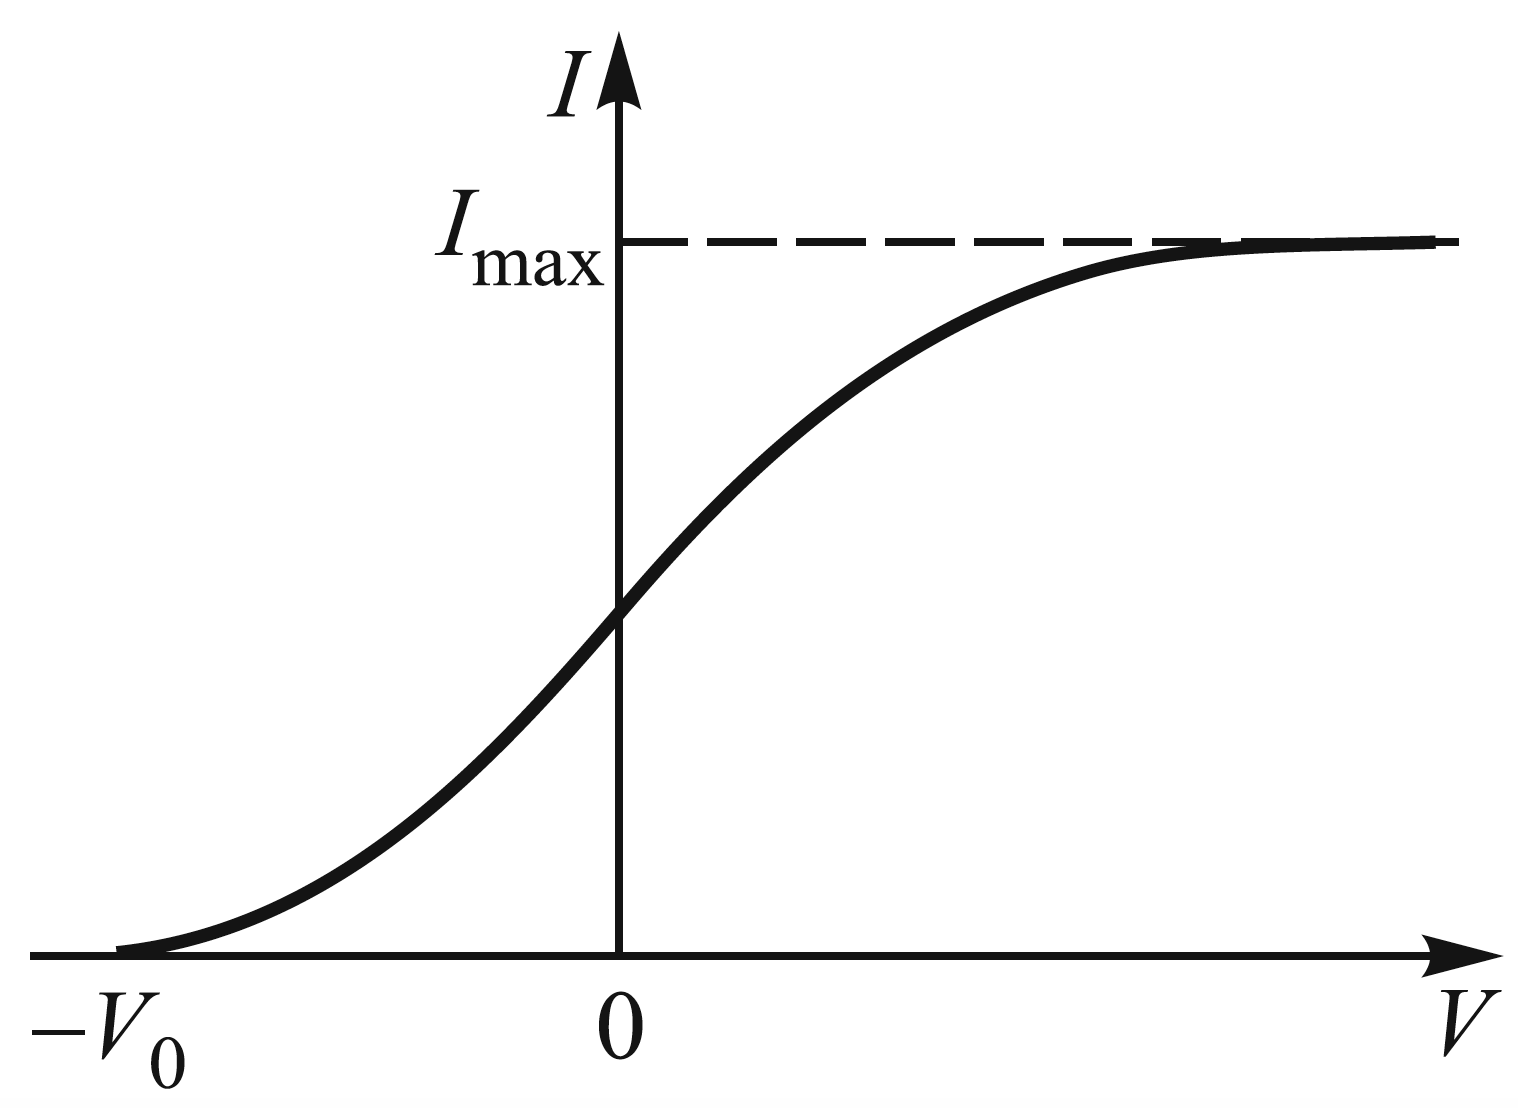
\includegraphics[width=\linewidth]{images/I(V).png}
		\caption{Зависимость фототока от напряжения на аноде фотоэлемента}
		\label{fig:I(V)}
	\end{wrapfigure}
	
	Здесь $E_{max}$ --  максимальная кинетическая энергия электрона после выхода из фотокатода, $W$ -- работа выхода электрона из катода. Реально энергетический спектр вылетевших из фотокатода электронов непрерывен -- он простирается от нуля до $E_{max}$. 
	
	Для измерения энергии вылетевших фотоэлектронов вблизи фотокатода обычно располагается второй электрод
	(анод), на который подается задерживающий ($V < 0$) или ускоряющий ($V > 0 $) потенциал. При достаточно больших
	ускоряющих напряжениях фототок достигает насыщения (рис. \ref{fig:I(V)}), и все испущенные электроны попадают на анод.
	
	При задерживающих потенциалах на анод попадают лишь электроны,
	обладающие достаточно большой кинетической энергией, в то время как медленно движущиеся электроны заворачиваются полем и возвращаются на катод. При некотором значении $V = -V_0$ (потенциал запирания) даже наиболее быстрые фотоэлектроны не могут достичь анода. Максимальная кинетическая энергия $E_{max}$ электронов связана с запирающим потенциалом $V_0$ очевидным соотношением $E_{max} = eV_0$, тогда \eqref{eq:energy} примет вид, называемый уравнением Эйнштейна:
	
	\begin{equation}
        \label{eq:Einsteain}
        eV_0 = \hbar\omega - W 
	\end{equation}
	
	Чтобы определить величину запирающего
	напряжения, нам надо правильно экстраполировать получаемую токовую зависимость к нулю, т.е. определить, какова функциональная зависимость $I(V)$. Расчет для простейшей геометрии -- плоский катод, освещаемый светом, и параллельный ему анод -- приводит к зависимости
	
	\begin{equation}
        \sqrt{I} \propto V_0 - V,
	\end{equation}
	
	т.е. корень квадратный из фототока линейно
	зависит от запирающего напряжения. Эта зависимость хорошо описывает экспериментальные данные.
    
    \newpage
    
    \section{Методика измерений и экспериментальная установка}

    \subsection{Описание экспериментальной установки}

    Схема экспериментальной установки приведена на рисунке \ref{img:installation_1}.
    
	\begin{figure}[H]
		\centering
		\begin{minipage}[c]{0.48\textwidth}
			\centering
			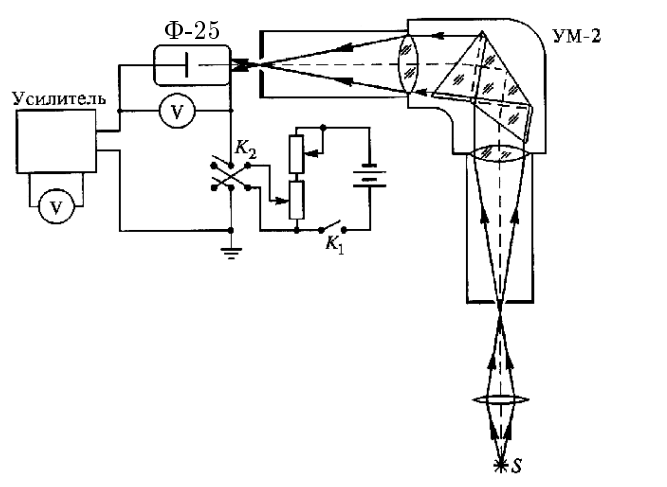
\includegraphics[width = 0.75\textwidth]{images/installation_1.png}
			\caption{Схема экспериментальной установки}
			\label{img:installation_1}
		\end{minipage}
		\hfill
		\begin{minipage}[c]{0.48\textwidth}
			\centering
			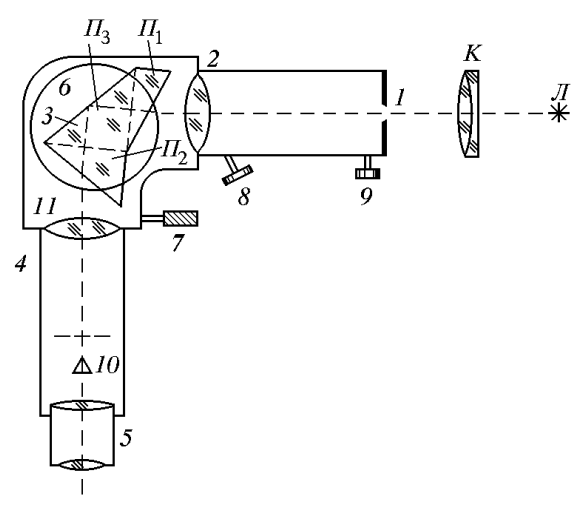
\includegraphics[width = 0.75\textwidth]{images/installation_2.png}
			\caption{Схема монохроматора.}
			\label{img:installation_2}
		\end{minipage}
	\end{figure}

	Излучения источника $S$ фокусируется на входную щель призменного монохроматора УМ-2, выделяющего узкий спектральный интервал, и попадает на катод фотоэлемента Ф-25.
	
	Рассмотрим схему монохроматора рисунок \ref{img:installation_2}. Входная щель 1 снабжена микрометрическим винтом 9 для регулировки нужной ширины щели. Коллиматорный объектив 2 имеет микрометрический винт 8, который позволяет смещать объектив относительно щели при фокусировке различных спектральных линий. Спектральная призма 3 выделяет узкую линию спектра падающего излучения. Поворотный столик 6 и барабан 7 с делениями позволяют наводиться на нужную спектральную линию. Зрительная труба, состоящая из объектива 4 и окуляра 5, позволяет проградуировать барабан на спектральные линии. При измерениях зрительная трубка заменяется блоком фотодетектора. 
	
	Фототок на фотоэлемента усиливается усилителем и напряжение, пропорциональное току измеряется вольтметром. Величина задерживающего напряжение фотоэлемента измеряется вторым вольтметром. Величину задерживающего напряжения можно регулировать с помощью блока питания.
 
    \subsection{Оборудование и приборы}

    \begin{itemize}	
        \item Цифровые мультиметры GDM-8145. В режиме измерения постоянного напряжения погрешность измерения оценивается по формуле 
        
        $$
        \pm (0.03\% \cdot \text{<измеренное значение>} + 4 \text{ единицы младшего разряда}).
        $$
        
        В режиме измерения постоянной силы тока на пределе $20 \A$ допустимое отклонение измеренных значений от реальных составляет 
        $$
        \pm (0.3\% \cdot \text{<измеренное значение>} + 2\text{ единицы младшего разряда}).
        $$

        \item Фотоэлемент Ф-25.
		
		\item Призменный монохроматор УМ-2. Рабочий диапазон от $0.38 \um$ до $1.00 \um$.
		
		\item Неоновая лампа.
		
		\item Лампа накаливания К-12.

        \item Блок питания.
    \end{itemize}

    \subsection{Методика эксперимента}

    В работе изучается зависимость фототока из фотоэлемента от величины задерживающего потенциала $V$ для различных частот света $\omega$, лежащих в видимой области спектра. С целью экспериментальной проверки уравнения Эйнштейна определяются потенциалы запирания $V_0$ при разных частотах света и строится зависимость $V_0(\omega)$, которая, как это следует из \eqref{eq:Einsteain}, должна иметь вид
	
	\begin{equation}
        \label{eq:V(w)}
        V_0 (\omega) = \frac{\hbar\omega - W}{e}
	\end{equation}

    \begin{figure}[H]
        \centering
        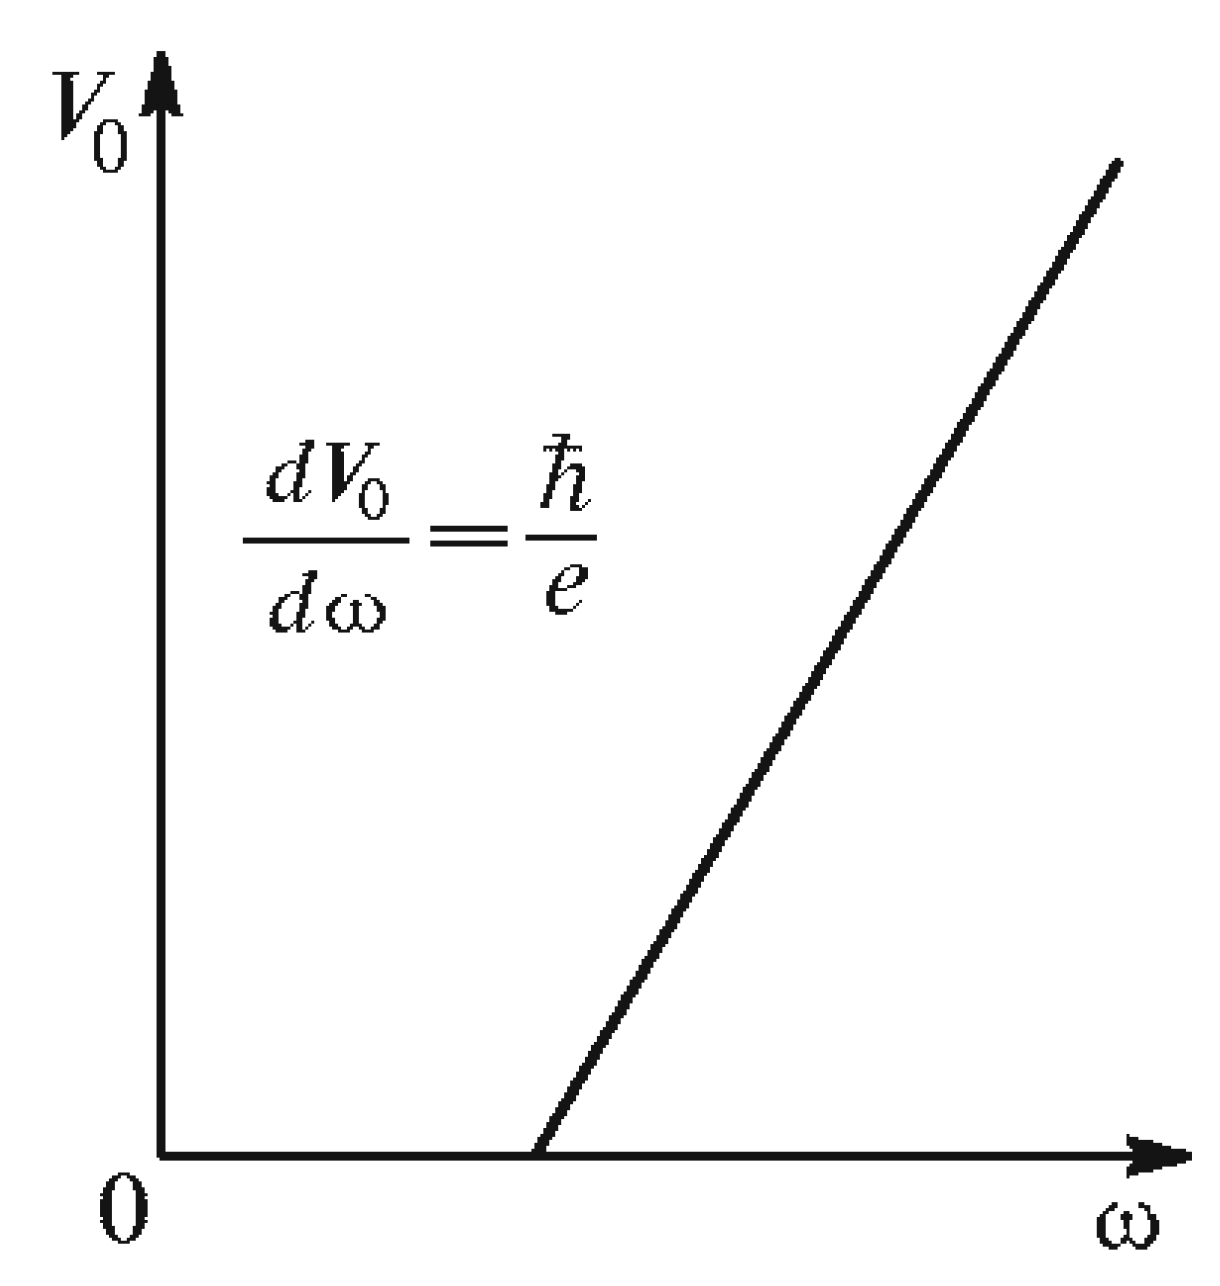
\includegraphics[width = 0.25 \textwidth]{images/V(w).png}
        \caption{Зависимость запирающего потенциала от частоты света}
        \label{fig:V(omega)}
    \end{figure}
	
	Потенциал запирания $V_0$ для любого катода линейно зависит от
	частоты света $ \omega $. По наклону прямой на графике $ V_0(\omega) $ (рис. \ref{fig:V(omega)}) можно определить постоянную Планка:
	
	\begin{equation}
        \label{eq:dV/dw}
        \frac{dV_0}{d\omega} = \frac{\hbar}{e}
	\end{equation}
	
	Как показывает формула \eqref{eq:dV/dw}, угол наклона прямой $V_0(\omega)$ не зависит от рода вещества, из которого изготовлен фотокатод. От рода вещества, однако, зависит величина фототока, работа выхода $W$ и форма кривой $I(V)$ (рис. \ref{fig:I(V)}). Все это определяет выбор пригодных для
	опыта катодов.

    \newpage
	
    \section{Результаты измерений и обработка данных}

    Сначала выполним градуировку монохроматора. Проведём серию измерений для линий спектра неона, снимая зависимость длины волны света от параметра $N$ барабана монохроматора. Построим график градуировочной кривой призменного монохроматора (рис. \ref{fig:calibration}).

    \begin{figure}[H]
        \centering
        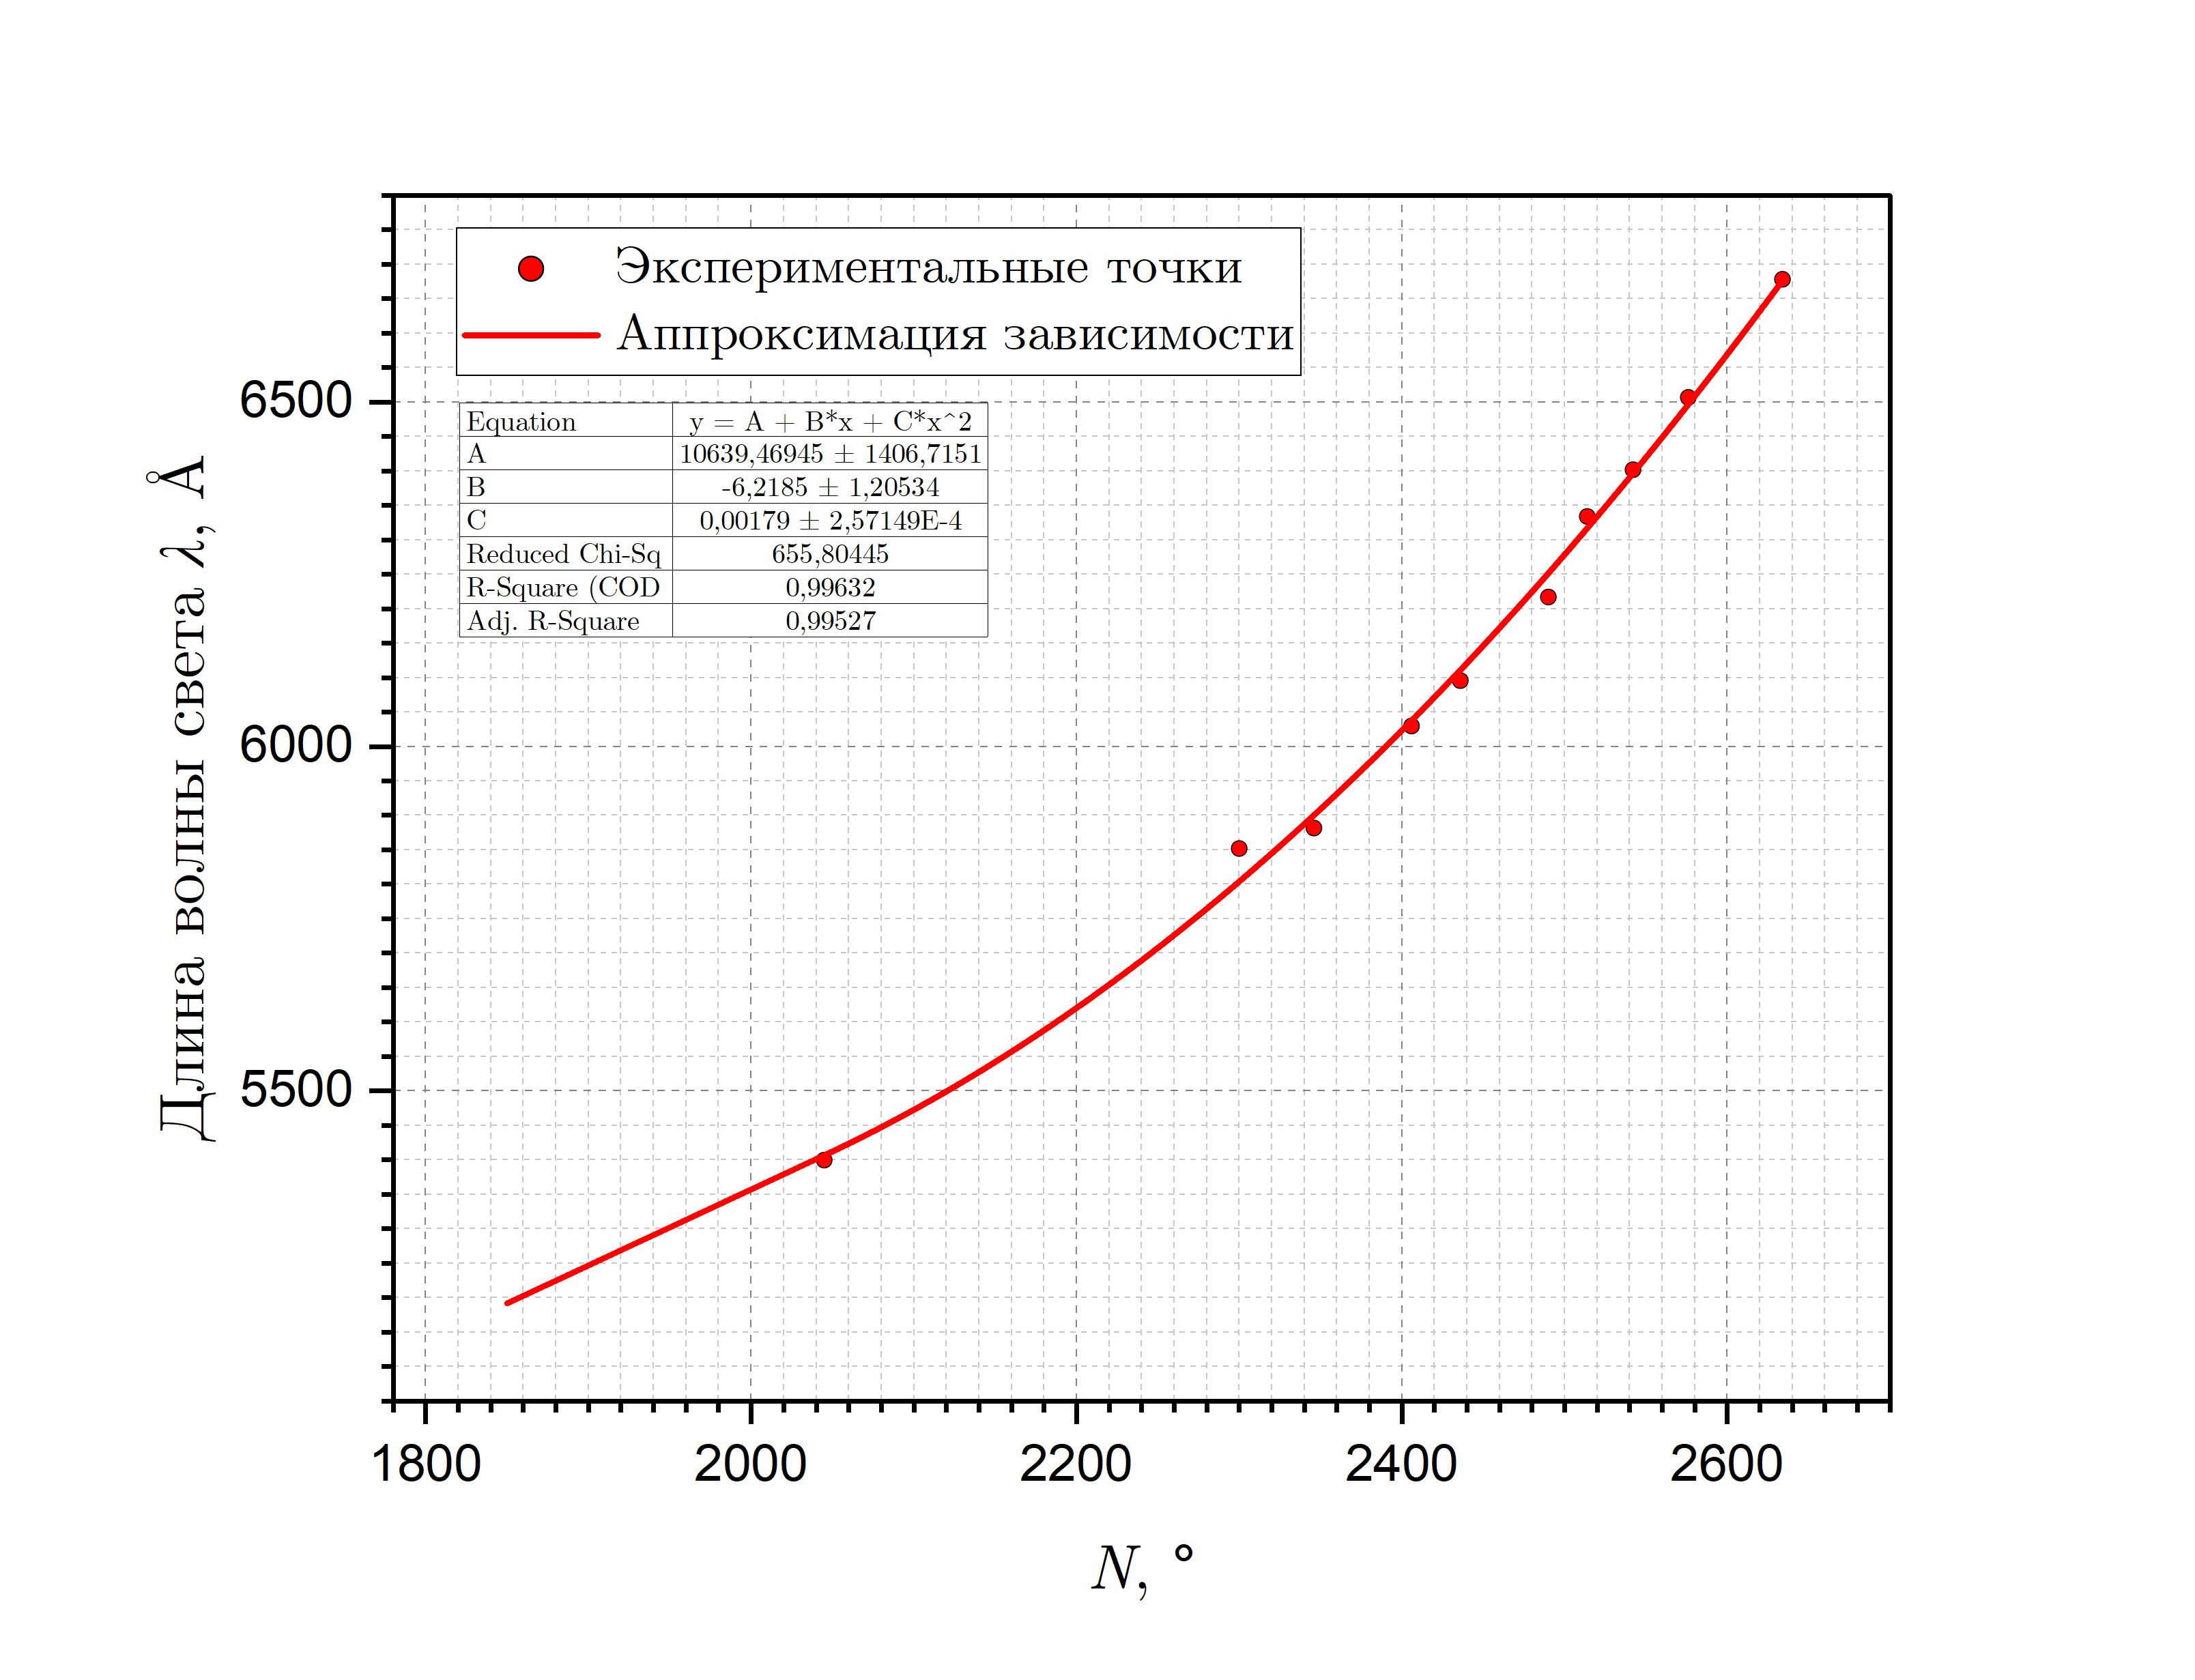
\includegraphics[width = 0.5\linewidth]{images/calibration_graph.png}
        \caption{Градуировочная кривая монохроматора}
        \label{fig:calibration}
    \end{figure}

    Погрешность измерения угла $\sigma_N = 2 ^\circ$. Длина спектральной линии является табличным значением, погрешностью её определения пренебрегаем.
    
    Видно, что график не является прямой и поэтому необходимо было провести градуировку: поставить в соответствие каждой спектральной линии угол, измеренный по отсчётному барабану.

    Построим графики зависимостей корня из напряжения, пропорционального току, от задерживающего напряжения $\sqrt{U_I} (V)$ (рис. \ref{fig:iv_graph}).

    \begin{figure}[H]
        \centering
        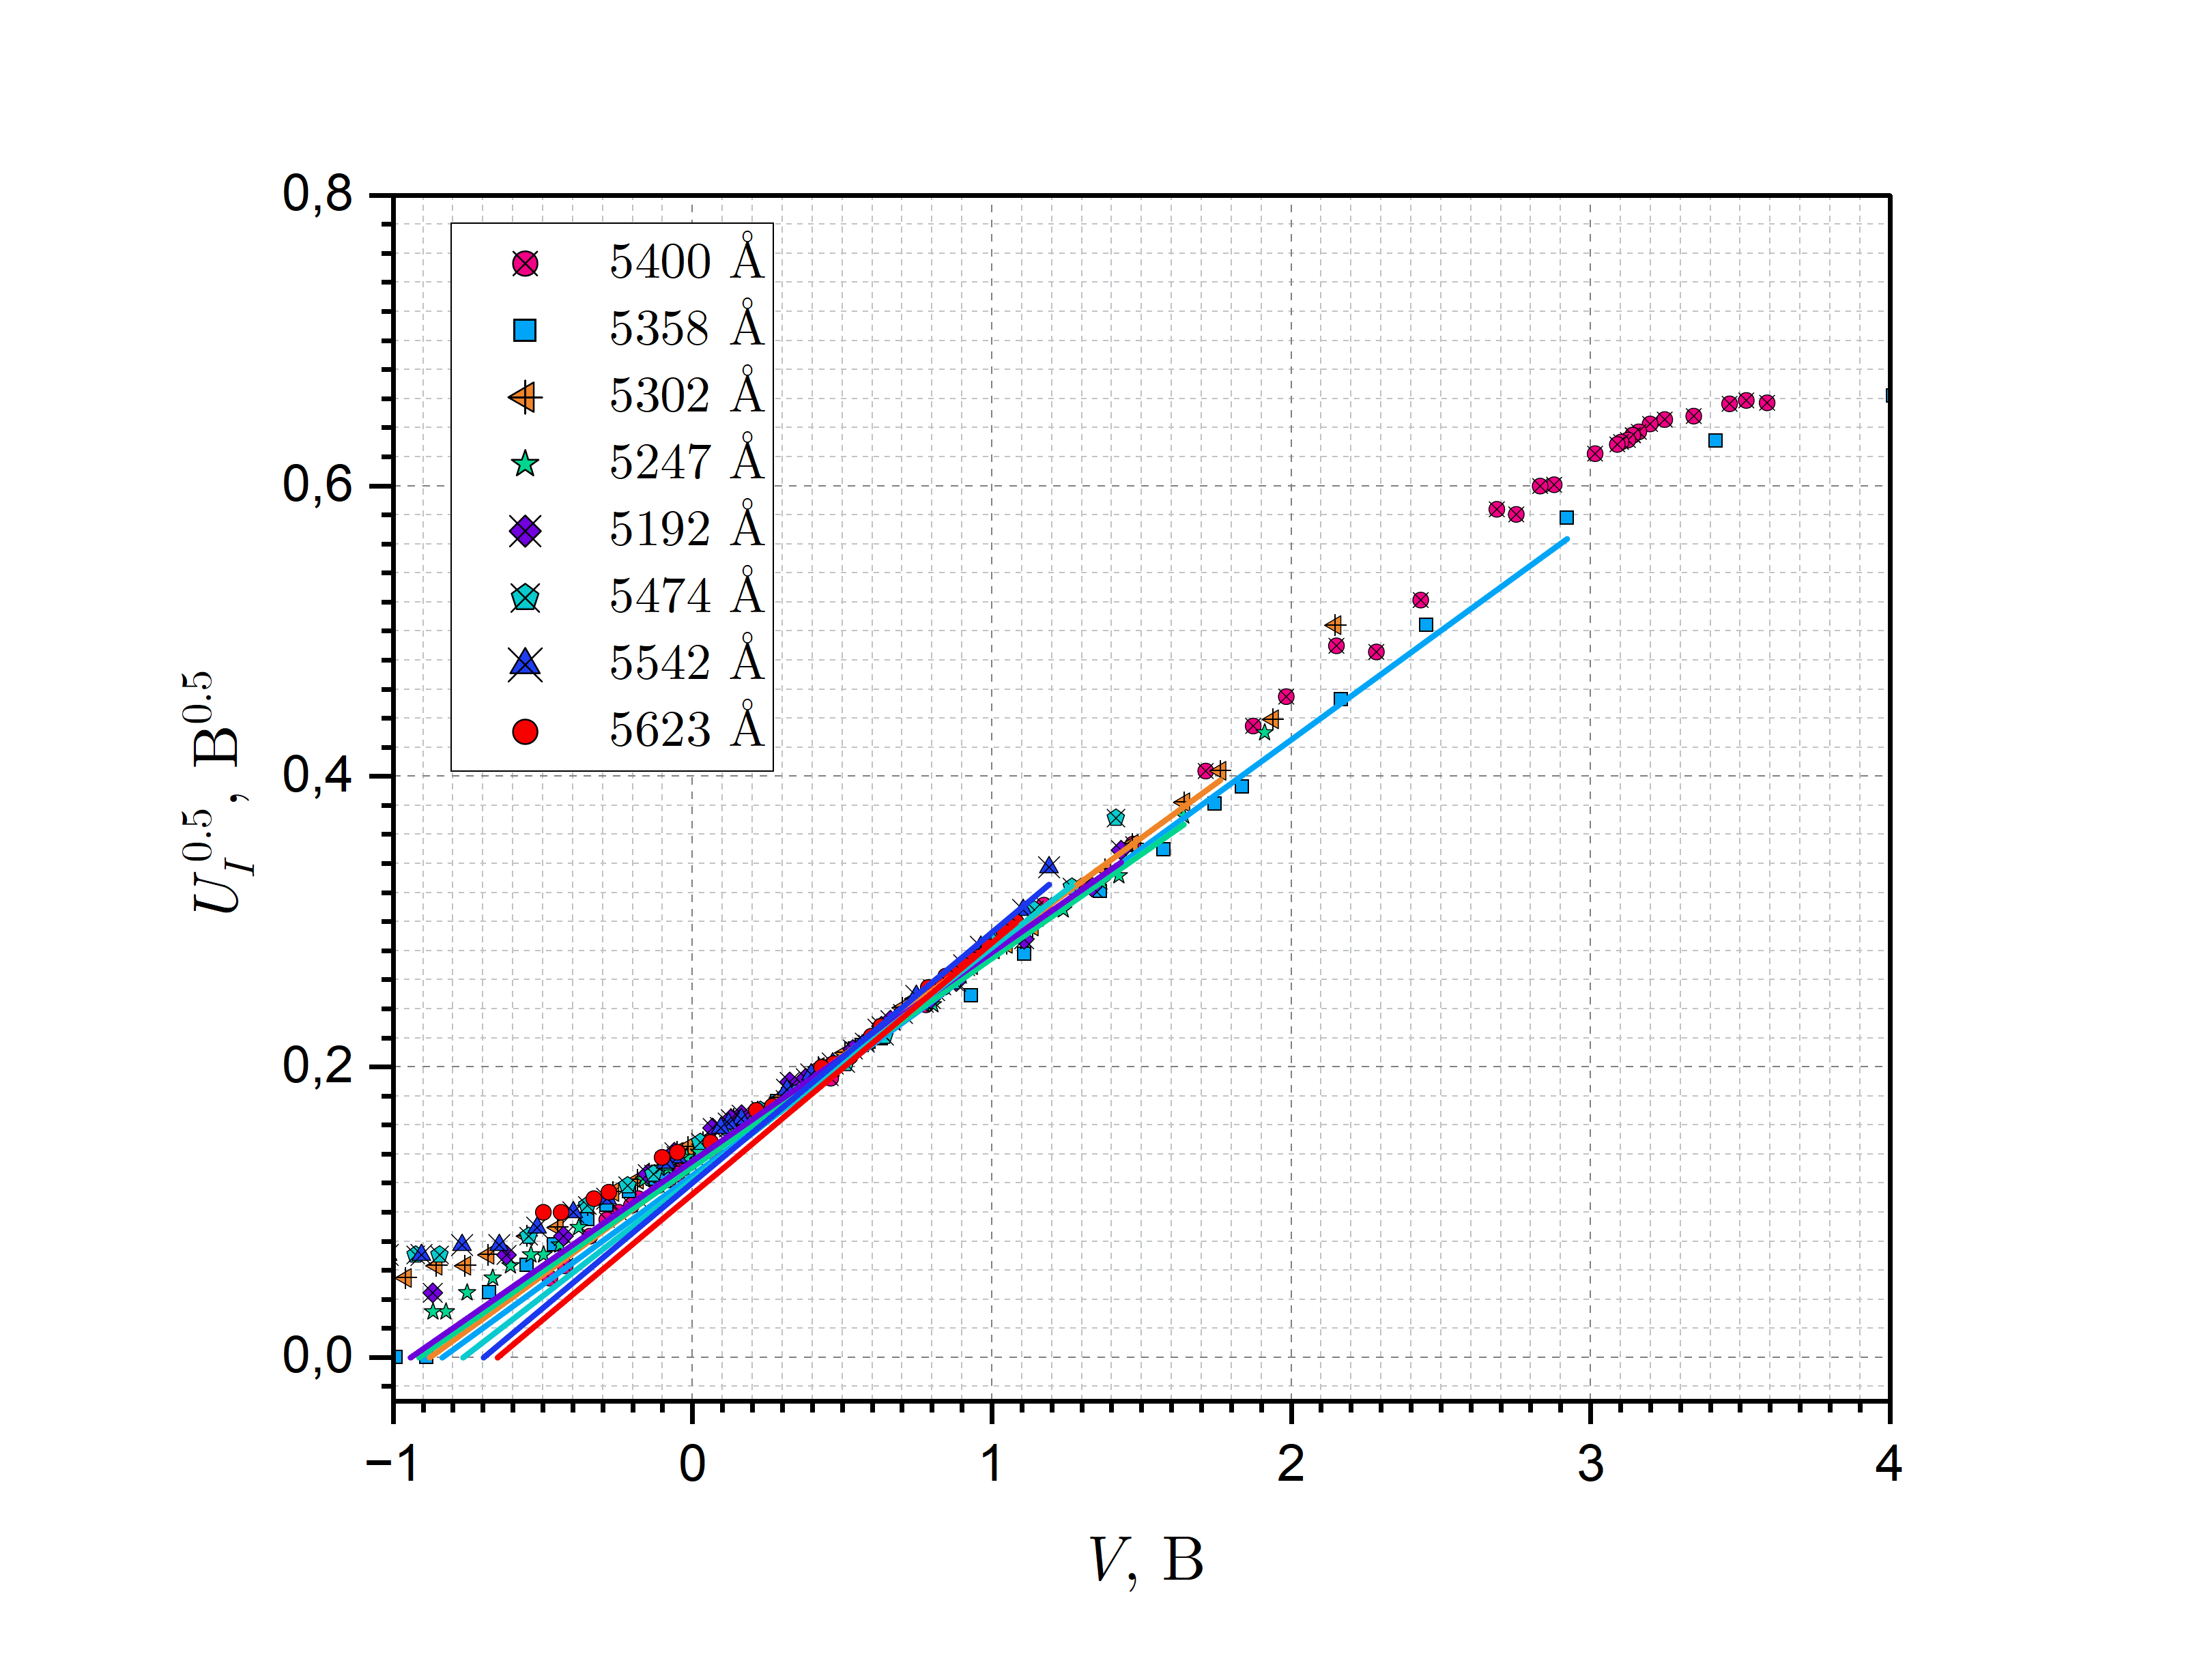
\includegraphics[width = 0.5\linewidth]{images/iv_graph.png}
        \caption{График зависимости $\sqrt{U_I} (V)$}
        \label{fig:iv_graph}
    \end{figure}

    Согласно теории $\sqrt{U_I} \propto V$. Методом наименьших квадратов построим аппроксимирующие кривые и определим величину задерживающего напряжения:
	
    \begin{table}[H]
        \centering
        \begin{tabular}{c}
            $\lambda = 5623 \angstrom, V_0 = - (0.65 \pm 0.02) В,$ \\
            $\lambda = 5542 \angstrom, V_0 = - (0.71 \pm 0.02) В,$ \\
            $\lambda = 5474 \angstrom, V_0 = - (0.77 \pm 0.02) В,$ \\
            $\lambda = 5400 \angstrom, V_0 = - (0.80 \pm 0.02) В,$ \\
            $\lambda = 5358 \angstrom, V_0 = - (0.84 \pm 0.03) В,$ \\   
            $\lambda = 5302 \angstrom, V_0 = - (0.87 \pm 0.03) В,$ \\
            $\lambda = 5247 \angstrom, V_0 = - (0.90 \pm 0.03) В,$ \\
            $\lambda = 5192 \angstrom, V_0 = - (0.95 \pm 0.04) В.$	
        \end{tabular}
    \end{table}

    Построим графики зависимостей ${U_I} (V)$ (рис. \ref{fig:iv_full_graph}).

    \begin{figure}[H]
        \centering
        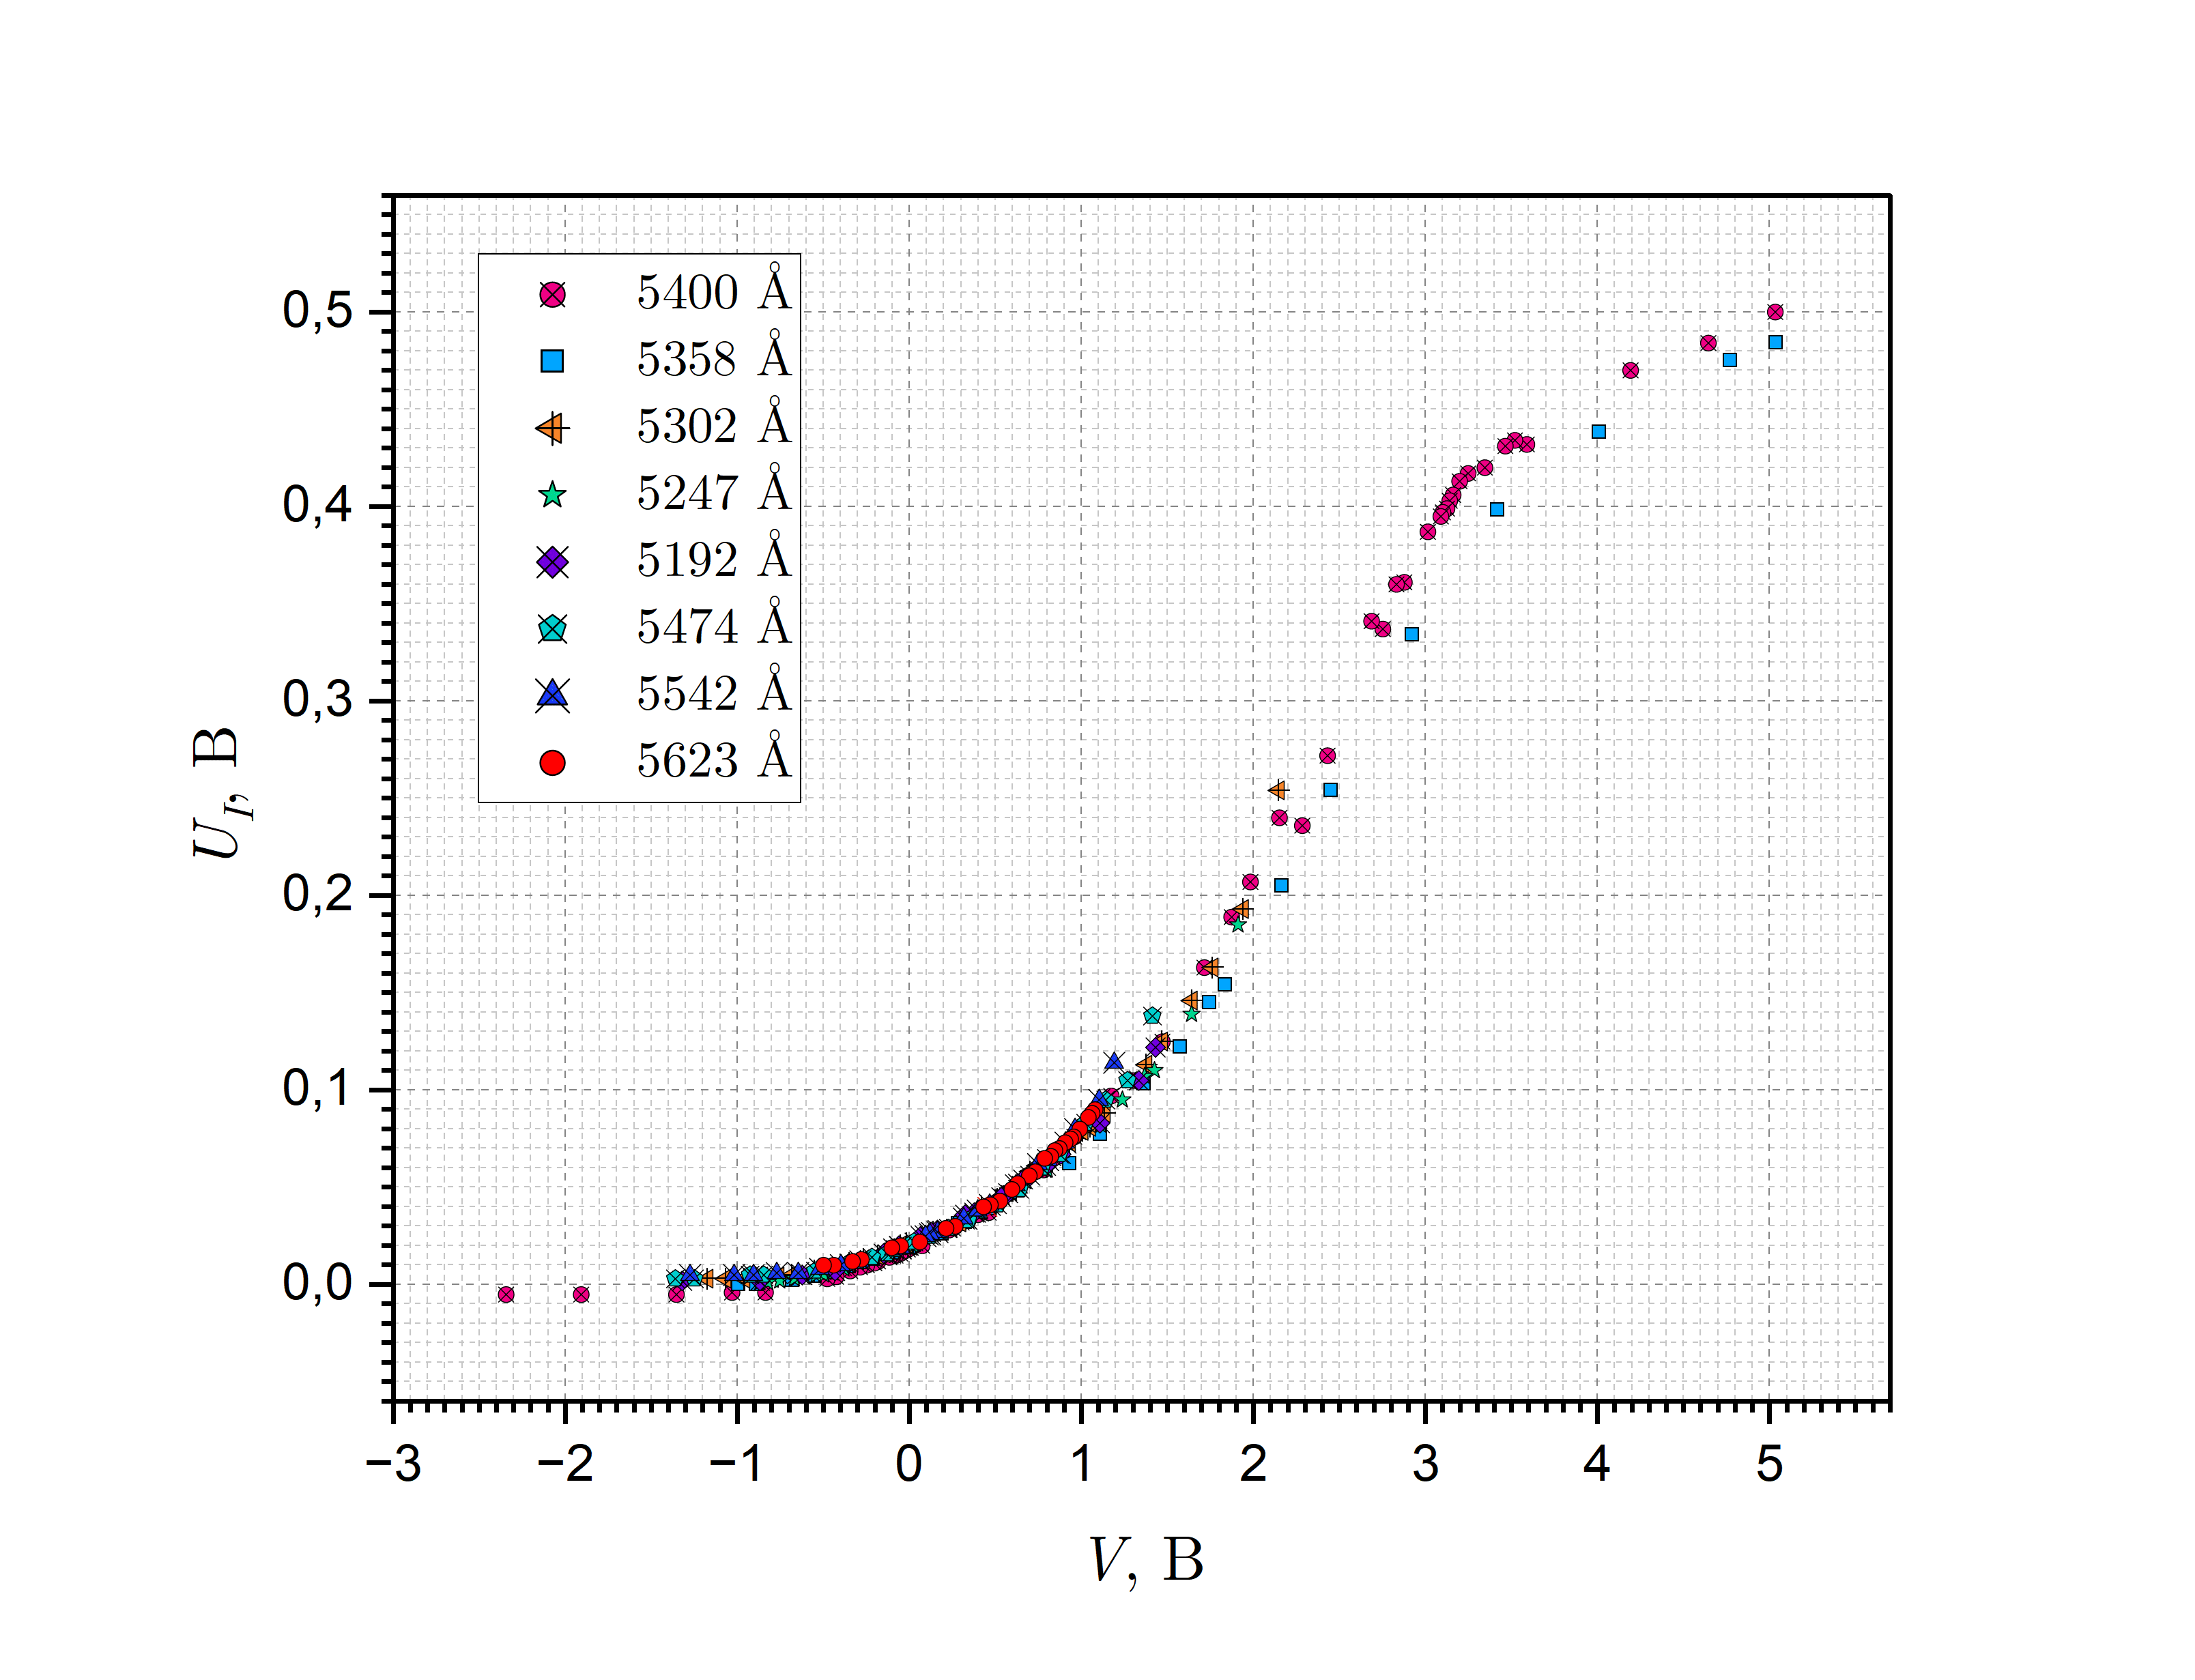
\includegraphics[width = 0.5\linewidth]{images/iv_full_graph.png}
        \caption{График зависимости ${U_I} (V)$}
        \label{fig:iv_full_graph}
    \end{figure}

    Видно, что с увеличением длины волны значение тока насыщения увеличивается, а величина запирающего потенциала уменьшается.

% Следующий график не получился из-за малого шага между измерениями в предыдущем пункте.

 %    Построим график зависимости задерживающего напряжения от частоты излучения (рис. \ref{fig:v0_omega}).
    
 %    \begin{figure}[H]
 %        \centering
 %        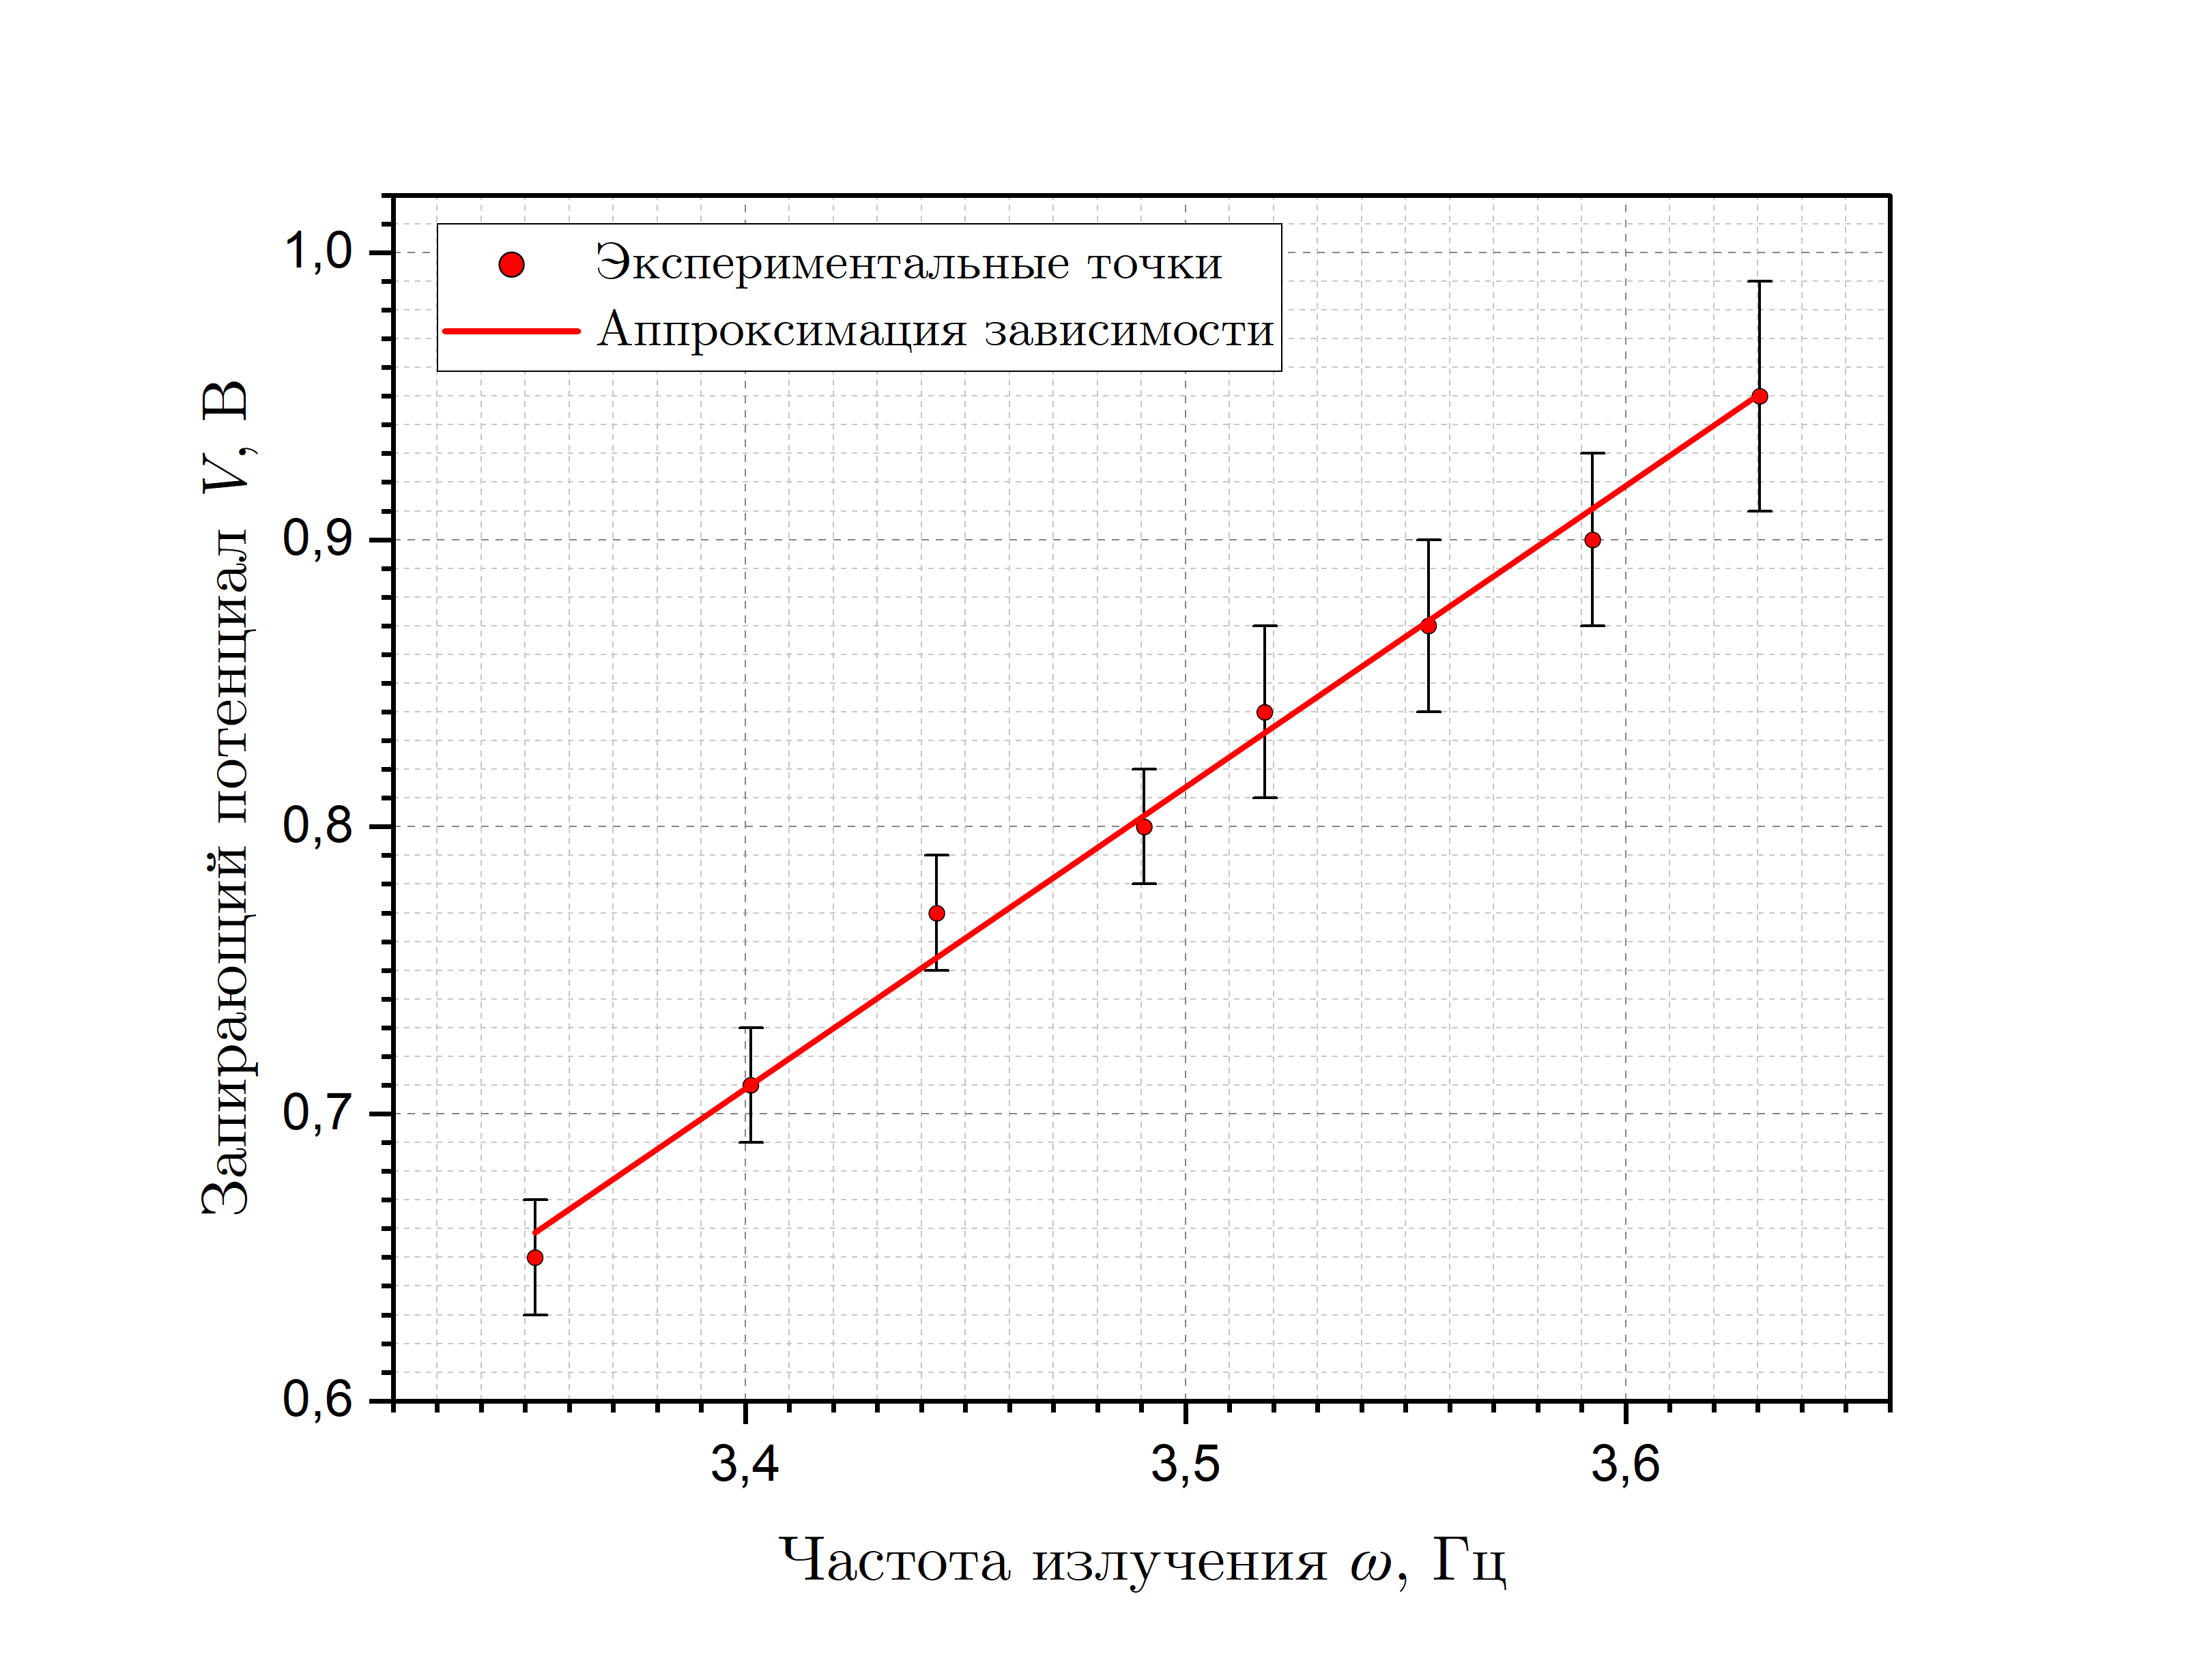
\includegraphics[width = 0.5\textwidth]{images/v0_omega_graph.png}
 %        \caption{График зависимости $U_0 (\omega)$}
 %        \label{fig:v0_omega}
 %    \end{figure}

	% С помощью метода наименьших квадратов проведём аппроксимирующую прямую. По коэффициенту наклона прямой $a$ определим постоянную Планка:
	% $\hbar = a \cdot e = (1.05 \pm 0.04) \cdot 10^{-34} \; Дж \cdot с.$
    
    \section{Заключение}
    
    \begin{itemize}
        \item В работе была экспериментально подтверждена линейная зависимость корня из фототока от величины запирающего потенциала:
    	$$
    	\sqrt{I} \propto V_{зап}.
    	$$

        \item Была подтверждена линейная зависимость запирающего потенциала от частоты падающего на фотоэлемент излучения:
    	$$
    	V_{зап} \propto \omega.
    	$$
    \end{itemize}
    
\end{document}